%-------------------------------------------------------------------------------
%-------------------------------------------------------------------------------
%-------------------------------------------------------------------------------
\chapter{Boucles 1 : for}
%-------------------------------------------------------------------------------
%-------------------------------------------------------------------------------
\thispagestyle{empty}
%-------------------------------------------------------------------------------
%-------------------------------------------------------------------------------
% {\sf Deux et deux quatre

% quatre et quatre huit

% huit et huit font seize \dots

% Répétez! dit le maître \hfill Jacques Prévert, Page d'écriture}

% \vfill

\begin{abstract} Dans ce T.P. nous allons mettre en œuvre la répétitions des instructions avec une boucle \Type{for}.
\end{abstract}
%-------------------------------------------------------------------------------
%-------------------------------------------------------------------------------
%-------------------------------------------------------------------------------
\section{Répétitions simples}
%-------------------------------------------------------------------------------
%-------------------------------------------------------------------------------
L'usage le plus simple d'une boucle \type{for} est de faire exécuter un certain nombre de fois les mêmes instructions. On emploie la structure \type{for i in range(n)} pour répéter $n$ fois, la variable $i$ n'est pas utilisée\footnote{On pourrait écrire \type{for \_ in range(n)}, le caractère "\_" représente une variable sans nom.}
%-------------------------------------------------------------------------------
%-------------------------------------------------------------------------------
\begin{Exercise}[title= La punition]
Écrire une fonction \type{ecrirePunition(texte,n)} qui reçoit deux paramètres
%-------------------------------------------------------------------------------
\begin{itemize}
\item \type{texte} est une chaîne de caractères
\item \type{n} est un entier
\end{itemize}
%-------------------------------------------------------------------------------
et qui écrit $n$ fois le texte à l'écran. Exceptionnellement, il n'y a pas de \type{return}.
\end{Exercise}
%-------------------------------------------------------------------------------
\begin{Answer}
\begin{lstlisting}
def ecrirePunition(texte,n):
	  """Entrées : une chaîne de caractères et un entier
	     Sortie  : la chaîne est écrite n fois"""
    for i in range(n):
        print(texte)
\end{lstlisting}
\end{Answer}
%-------------------------------------------------------------------------------
%-------------------------------------------------------------------------------
\begin{Exercise}[title= Une suite]
Écrire une fonction \type{heron(n, u0)} qui calcule (et renvoie) le terme $u_n$ de la suite $(u_p)$ définie par $u_0=$\ \type{u0} et $u_{p+1} = \frac 12\bigl(u_p + \frac 2{u_p}\bigr)$ (suite de Héron).
\end{Exercise}
%-------------------------------------------------------------------------------
\begin{Answer}
\begin{lstlisting}
def heron(n,u0):
	  """Entrées : un entier positif n et un réel u0
	     Sortie  : le n-ième terme de la suite de Héron"""
    u = u0
    for i in range(n):
        u = (u + 2/u)/2
    return u
\end{lstlisting}
\end{Answer}
%-------------------------------------------------------------------------------
%-------------------------------------------------------------------------------
\begin{Exercise}[title= Suite de Fibonacci : 1]
On considère la suite (de Fibonacci) définie par $F_{0}=0$, $F_1=0$ et $F_{n+2}=F_{n+1}+F_{n}$ pour $n\ge 0$.

Écrire un programme \texttt{fibo(n)} qui renvoie $F_n$.

{\it On pourra maintenir deux variables qui correspondent à 2 valeurs consécutives de la suite.}
\end{Exercise}
%-------------------------------------------------------------------------------
\begin{Answer}
\begin{lstlisting}
def fibo(n):
    """Entrée : un entier positif n
	   Sortie : le n-ième nombre de Fibonacci"""
    F = 0
    F_suivant = 0
    for i in range(n): # On calcule les couples (F1, F2), (F2, F3), ..., (Fn,F(n+1))
        F_vieux = F
        F = F_suivant
        F_suivant = F + F_vieux
    return F
\end{lstlisting}

Il est à noter que l'on a calculé un terme de plus : on pourrait être tenté d'écrire
\begin{lstlisting}
def fibo(n):
    """Entrée : un entier positif n
	   Sortie : le n-ième nombre de Fibonacci"""
    F = 0
    F_suivant = 0
    for i in range(n-1): # On calcule les couples (F1, F2), (F2, F3), ..., (F(n-1), Fn)
        F_vieux = F
        F = F_suivant
        F_suivant = F + F_vieux
    return F_suivant
\end{lstlisting}
La valeur de \type{fibo(0)} serait juste mais uniquement car $F_0=F_1$..
\end{Answer}
%-------------------------------------------------------------------------------
%-------------------------------------------------------------------------------
\section{Utilisation de l'indice de boucle}
%-------------------------------------------------------------------------------
%-------------------------------------------------------------------------------
\begin{Exercise}[title= Table de multiplication]
Écrire une fonction \type{table(n} qui écrit la table de multiplication par $n$.

\begin{lstlisting}
1 fois 7 donne 7
2 fois 7 donne 14
...
\end{lstlisting}
\end{Exercise}
%-------------------------------------------------------------------------------
\begin{Answer}
\begin{lstlisting}
def table(n):
   for k in range(1, 11):
       print("{} fois {} donne {}.format(n, k, k*n))
\end{lstlisting}
\end{Answer}
%-------------------------------------------------------------------------------
%-------------------------------------------------------------------------------
\begin{Exercise}[title= Suite de Fibonacci : 2]
Affichez les valeurs de $F_0$ à $F_{12}$. 
\end{Exercise}
%-------------------------------------------------------------------------------
\begin{Answer}
\begin{lstlisting}
for i in range(13):
    print("F{} vaut {}".format(i, fibo(i)))
\end{lstlisting}
\end{Answer}
%-------------------------------------------------------------------------------
%-------------------------------------------------------------------------------
\begin{Exercise}[title= Suite harmonique, label=exo:harmo]
Écrire une fonction \type{harmo(n)} qui renvoie $\displaystyle \sum_{k=1}^n \frac 1k$ (pour $n\ge 1$).
\end{Exercise}
%-------------------------------------------------------------------------------
\begin{Answer}
\begin{lstlisting}
def harmo(n) :
	  """Entrée : un entier strictement positif
	     Sortie : la valeur de Hn"""
    h=0
    for k in range(n):
        h = h + 1/(k+1)
    return k
\end{lstlisting}
\end{Answer}
%-------------------------------------------------------------------------------
%-------------------------------------------------------------------------------
\begin{Exercise}[title= Factorielle]
Écrire une fonction \type{facto(n)} qui renvoie $n!$.

Utiliser cette fonction pour écrire une fonction \type{binomial(n,p)} qui renvoie $\displaystyle\binom np$.
\end{Exercise}
%-------------------------------------------------------------------------------
\begin{Answer} Il faut initialiser par 1 car on fait des produits.
\begin{lstlisting}
def facto(n):
	  """Entrée : un entier positif
	     Sortie : la valeur de n!"""
    f = 1
    for k in range(n):
        f = f*(k+1)
    return f
\end{lstlisting}

\begin{lstlisting}
def binomial(n,p):
    return facto(n)//facto(p)//facto(n-p)
\end{lstlisting}

\end{Answer}
%-------------------------------------------------------------------------------
%-------------------------------------------------------------------------------
\begin{Exercise}[title= {Coefficients binomiaux, bis}]
La fonction précédente manipule des entiers qui peuvent être beaucoup plus grands que le résultat.

Si on n'a pris soin d'écrire des divisions entières (//) \type{binomial(1000, 1)} donne une erreur.

Écrire une fonction \type{binomial(n,p)} qui renvoie $\displaystyle\binom np$ en utilisant la propriété $\displaystyle  \binom n{k+1} = \frac{n-k}{k+1} \binom nk$.
\end{Exercise}
%-------------------------------------------------------------------------------
\begin{Answer} 
\begin{lstlisting}
def binomial1(n, p):
    b = 1
    for k in range(p):
        b = b * (n-k) // (k+1)
    return b
\end{lstlisting}
\end{Answer}
%-------------------------------------------------------------------------------
%-------------------------------------------------------------------------------
\begin{Exercise}[title= Somme de puissances]
Écrire une fonction \type{sommePuissances(n,p)} qui renvoie $\displaystyle \sum_{k=1}^n k^p$.

Calculer, pour quelques valeurs de $n$, 
\type{sommePuissances(n,3)-(sommePuissances(n,1))**2}.
\end{Exercise}
%-------------------------------------------------------------------------------
\begin{Answer} 
\begin{lstlisting}
def sommePuissances(n,p):
	  """Entrées : deux entiers positifs
	     Sortie  : la valeur de sum(k^p,k=1..n)"""
    s=0
    for k in range(1, n+1):
        s = s + k**p
    return s
\end{lstlisting}

\begin{lstlisting}
for n in range(1, 11):
   print("La somme des cubes de 1 à {} vaut {}".format(n,sommePuissances(n,3)))
   print("La somme des entiers de 1 à {} au carré vaut {}".format(n,(sommePuissances(n,3))**2))
\end{lstlisting}
\newpage
\end{Answer}
%-------------------------------------------------------------------------------
%-------------------------------------------------------------------------------
\begin{Exercise}[title= Série]

On veut étudier la suite défine par la somme $\displaystyle S_n=\sum_{k=0}^n \frac{2^k}{k!}$.
\begin{itemize}
    \item Écrire une fonction \type{a(n)} qui calcule $a_n=\frac{2^n}{n!}$ ; en déduire une fonction \type{S(n)} qui calcule $S_n$. Combien d'opérations sont effectuées lors de l'appel de \type{S(n)} ?
    \item Proposer une fonction \type{S1(n)} qui calcule $S_n$ en effectuant un nombre d'opération proportionnel à $n$ (en fait proportionnel à $n+1$).
\end{itemize}
\end{Exercise}
%-------------------------------------------------------------------------------
\begin{Answer} 
\begin{itemize}
\item 
\begin{lstlisting}
def a(n):
    terme = 1
    for i in range(n):
        terme = terme*2/(i+1)
    return terme

def S(n):
    somme = 0
    for k in range(n+1):
        somme = somme + a(k)
    return somme
\end{lstlisting}
L'appel de \type{a(k)} effectue $2k$ opérations donc l'appel de \type{S(n)} effectue

$\displaystyle C(n) = \sum_{k=0}^n 1+2k = n+1+2\sum_{k=0}^nk=(n+1)^2$ opérations.
%-------------------------------------------------------------------------------
\item On calcule $a_n$ dans la boucle
\begin{lstlisting}
def S1(n):
    a = 1
    somme = 0
    for k in range(n+1):
        somme = somme + a
        a = a*2/(k+1)
    return somme
\end{lstlisting}
On effectue maintenant $\displaystyle C_1(n) = \sum_{k=0}^n 3 = 3(n+1)$ opérations.
\end{itemize}
\end{Answer}
%-------------------------------------------------------------------------------
%-------------------------------------------------------------------------------
\begin{Exercise}[title= Constante d'Euler]

Les deux suites $(u_n)_{n\ge 1}$ et $(v_n)_{n\ge 1}$ définies par $u_n = H_n -\ln(n+1)$ et $v_n = H_n -\ln(n)$ (voir ref{exo:harmo}) sont adjacentes ; leur limite commune est la constante d'Euler, notée $\gamma$. On a donc $u_n \le \gamma \le v_n$ pour tout $n$.

On prouve, de plus qu'on a $v_n - u-n \le \frac 1n$.

Écrire une fonction \type{gamma(e)} qui calcule un encadrement de $\gamma$ avec une précision $e$.
\end{Exercise}
%-------------------------------------------------------------------------------
\begin{Answer} 
\begin{lstlisting}
import math as m
def gamma(e):
    n = int(1/e) + 1
    h = 0
    for k in range(1, n+1):
        h = h + 1/k
    return h - m.log(n+1), h - m.log(n)
\end{lstlisting}
\end{Answer}
%-------------------------------------------------------------------------------
%-------------------------------------------------------------------------------
\subsection{Suite de Muller (1993)}
%-------------------------------------------------------------------------------
%-------------------------------------------------------------------------------
{\it La suite de {\sc Muller} est définie par
$\displaystyle u_0 = \frac 52,\ u_1 = \frac{17}5 \text{ et }u_{n+2} = 30 - \frac {129}{u_{n+1}} + \frac {100}{u_n.u_{n+1}}\text{ pour }n\ge 0$.}
%-------------------------------------------------------------------------------
%-------------------------------------------------------------------------------
\begin{Exercise}[title= Calcul des termes] 
Écrire une fonction \type{muller(n)} qui calcule le terme $u_n$ de cette suite.

Calculer les 50 premières valeurs de $u_n$ ; quelle semble être la limite ?
\end{Exercise}
%-------------------------------------------------------------------------------
\begin{Answer}
\begin{lstlisting}
def muller(n):
    u = 5/2
    u_suivant = 17/5
    for i in range(n):
        u_avant = u
        u = u_suivant
        u_suivant = 30 - 129/u + 100/u/u_avant
    return u
\end{lstlisting}

Dans la partie principale.
\begin{lstlisting}
for k in range(50):
    print("u{} vaut {}".format(k, muller(k)))
\end{lstlisting}

La suite semble converger vers 25 alors qu'elle semblait s'approcher de 4 au début.
\end{Answer}
%-------------------------------------------------------------------------------
%-------------------------------------------------------------------------------
{\it On prouve, par récurrence, que $\displaystyle u_n = \frac{1+4^{n+1}}{1+4^{n}}$ : la suite converge vers 4.

On peut utiliser des fractions ; elles sont utilisables comme les nombres.}
\begin{lstlisting}
from fractions import Fraction
a = Fraction(2, 6)
print(a, a*2, float(a))
\end{lstlisting}
%-------------------------------------------------------------------------------
%-------------------------------------------------------------------------------
\begin{Exercise}[title={Usage des fractions}]
Écrire une fonction \type{muller\_frac(n)} qui calcule le terme $u_n$ de la suite de Muller en utilisant les fractions.
\end{Exercise}
%-------------------------------------------------------------------------------
\begin{Answer} Il suffit de changer les termes initiaux
\begin{lstlisting}
def muller_frac(n):
    u = Fraction(5, 2)
    u_suivant = Fraction(17, 5)
    for i in range(n):
        u_avant = u
        u = u_suivant
        u_suivant = 30 - 129/u + 100/u/u_avant
    return u

for k in range(50):
    print("u{} vaut {}, {} sous forme décimale".format(k, muller_frac(k), float(muller_frac(k))))
\end{lstlisting}
\end{Answer} 
%-------------------------------------------------------------------------------
%-------------------------------------------------------------------------------
%-------------------------------------------------------------------------------
\section{Exercices supplémentaires}
%-------------------------------------------------------------------------------
%-------------------------------------------------------------------------------
%-------------------------------------------------------------------------------
Ces exercices sont destinés à ceux qui auraient achevé les 4 premiers T.P. et désireraient s'exercer sur des problèmes plus difficiles.
%-------------------------------------------------------------------------------
%-------------------------------------------------------------------------------
\subsection{Polynômes de degré 3, reprise du TP02}
%-------------------------------------------------------------------------------
%-------------------------------------------------------------------------------
Le but de ces exercices est de déterminer les 3 racines (complexes) d'un polynôme de degré 3 : $P(X)=X^3+aX^2++bX+c$. Même dans le cas d'un polynôme à coefficients réels et dont les 3 racines sont réelles ont doit calculer des valeurs intermédiaires complexes. 

On peut définir un nombre complexe à partir de son module $r$ et de son argument $\varphi$ à l'aide de la fonction \type{cmath.rect(r, phi)} du module \type{cmath}.
\begin{lstlisting}
import cmath 

>>> cmath.rect(2, cmath.pi/3)
(1.0000000000000002+1.7320508075688772j)
\end{lstlisting}

Il sera pratique de placer les racines dans une liste \type{r = [0]*3} dont les éléments seront accessibles par \type{r[0]}, \type{r[1]} et  \type{r[2]}. 

%-------------------------------------------------------------------------------
%-------------------------------------------------------------------------------
\begin{Exercise}
\it Écrire une fonction \type{racine3(u)} qui renvoie les 3 racines (complexes) de $u$.

Si $a_1$ est la valeur calculée par \type{u**(1/3)}, les deux autres racines sont $a_2=a_1e^{2i\pi/3}$ et $a_3=a_1e^{4i\pi/3}$ 
\end{Exercise}
%-------------------------------------------------------------------------------
\begin{Answer}
\begin{lstlisting}
def racines3(u):
    r = [0]*3
    v = u**(1/3)
    w = cmath.rect(1, 2*cmath.pi/3)
    for i in range(3):
        r[i] = v*w**i
    return r
\end{lstlisting}
\end{Answer}
%-------------------------------------------------------------------------------
%-------------------------------------------------------------------------------
\medskip

Dans le cas du polynôme $P(X)=X^3+pX+q$ on démontre (exercice de mathématique) que si on pose $X = a+b$ en imposant $ab = -\frac p3$ alors $a^3+b^3 = -q$. Comme on a aussi $a^3b^3 = -\frac {p^3}{27}$ on voit que $a^3$ et $b^3$ sont les racines de $\displaystyle Q(X) = X^2 +qX-\frac {p^3}{27}$.

On obtient alors 2 racines $r_1$ et $r_2$. On démontre aussi que si

\begin{itemize}
    \item on choisit une des racines, $r_1$
    \item on attribue successivement à $a$ les 3 racines de $r_1$ comme valeur,
    \item on détermine $b$ par $ab = -\frac p3$,
\end{itemize} 

on obtient alors les trois racines de $P$ en calculant $a+b$.
%-------------------------------------------------------------------------------
%-------------------------------------------------------------------------------
\begin{Exercise}
\it Écrire une fonction \type{solutions1(p, q)} qui calcule les 3 racines du polynôme $X^3+pX+q$. On supposera $p$ non nul.
\end{Exercise}
%-------------------------------------------------------------------------------
\begin{Answer}
\begin{lstlisting}
def solutions1(p, q):
    delta  = q**2 + 4*p**3/27
    u = (-q + delta**(1/2))/2
    r = racines3(u)
    for i in range(3):
        r[i] = r[i] -p/(3*r[i])
    return r
\end{lstlisting}
\end{Answer}
%-------------------------------------------------------------------------------
%-------------------------------------------------------------------------------
\begin{Exercise}
 Dans le cas général, $P(X)=X^3+a X^2+ b X+ c$, montrer que $u$ est racine de $P$ si et seulement si $u+\frac a 3$ est racine d'un polynôme de la forme $P_1(X)=X^3+pX+q$ dont on déterminera les coefficients $p$ et $q$ en fonction de $a$, $b$  et $c$.
\end{Exercise}
%-------------------------------------------------------------------------------
\begin{Answer}

$\bigl(u+\frac a 3\bigr)^3 = u^3+a.u^2+\frac {a^2}3u+\frac {a^3}{27}$ or $u^3+a.u^2 = -\b.u-c$ car $u$ est racine.

Ainsi $\bigl(u+\frac a 3\bigr)^3 = \bigl(\frac {a^2}3 - a)u+\frac {a^3}{27}-c
=\bigl(\frac {a^2}3 - b)\bigl(u+\frac a3\bigr)+\frac {a^3}{27}-c-\frac {a^3}9+\frac{a.b}3$.

$p = b - \frac {b^2}3$ et $q = c - \frac{a.b}3+\frac {2a^3}{27}$.
\end{Answer}
%-------------------------------------------------------------------------------
%-------------------------------------------------------------------------------
\begin{Exercise}
\it En déduire une fonction \type{solutions(a, b, c)} qui calcule les 3 racines du  polynôme $P = X^3 + aX^2+ bX + c$.
\end{Exercise}
%-------------------------------------------------------------------------------
\begin{Answer}
\begin{lstlisting}
def solutions(a, b, c):
    p = b - a**2/3
    q = c - a*b/3 + 2*a**3/27
    d = -a/3
    if p == 0:
        r = racines3(-q)
    else:
        r = solutions1(p, q)
    for i in range(3):
        r[i] = r[i] + d
    return r 
\end{lstlisting}
\newpage
\end{Answer}
%-------------------------------------------------------------------------------
%-------------------------------------------------------------------------------
\subsection{6400 carrés dans un presque-carré}
%-------------------------------------------------------------------------------
%-------------------------------------------------------------------------------
{\sf Ce problème est le défi Turing 8 : http://apprendre-en-ligne.net/}

Dans un rectangle de longueur 4 et de largeur 3, on peut dessiner 12 carrés de côté 1, 6 carrés de côté 2 et 2 carrés de côté 3. Au total, on peut dessiner 20 carrés. Nous dirons que c'est un rectangle-20.
Les dimensions sont entières tant pour le rectangle que pour les carrés.

%-------------------------------------------------------------------------------
%-------------------------------------------------------------------------------
\begin{Exercise}
\it Quelle est l'aire du rectangle-6400 dont la forme est la plus proche d'un carré ?
\end{Exercise}
%-------------------------------------------------------------------------------
\begin{Answer}
\begin{lstlisting}
def carres(n, p):
    m = min(n, p)
    nb = 0
    for k in range(1, m + 1):
        nb = nb + (n + 1 - k)*(p + 1 - k)
    return nb

for i in range(1, 100):
    for j in range(i, 100):
        if carres(i, j) == 6400:
            print(i, j, i*j)
\end{lstlisting}
696
\end{Answer}
%-------------------------------------------------------------------------------
%-------------------------------------------------------------------------------
\subsection{Longue suite de Syracuse}
%-------------------------------------------------------------------------------
%-------------------------------------------------------------------------------
{\sf Ce problème est le défi Turing 14 : http://apprendre-en-ligne.net/

Il est aussi le problème 14 du Project Euler : https://projecteuler.net/problem=14}

La suite de Syracuse est définie par $u_0\in \N^*$ et 
$\displaystyle u_{n+1} =\left\{\begin{matrix} u_n/2&\text{si $u_n$ est pair}\\ 3u_n + 1&\text{si $u_n$ est impair} 
\end{matrix}\right.$

On conjecture que la suite de Syracuse de n'importe quel entier strictement positif atteint 1.

Par exemple, à partir de 14, on construit la suite des nombres : 

14, 7, 22, 11, 34, 17, 52, 26, 13, 40, 20, 10, 5, 16, 8, 4, 2, 1. 

C'est ce qu'on appelle la suite de Syracuse du nombre 14. Elle a ici une longueur de 18.
%-------------------------------------------------------------------------------
%-------------------------------------------------------------------------------
\begin{Exercise}
\it Pour quel nombre de départ inférieur à 1 500 000 obtient-on la plus longue suite de Syracuse ? Il y a deux solutions, donner la plus petite.
\end{Exercise}
%-------------------------------------------------------------------------------
\begin{Answer}
\begin{lstlisting}
def longueur(n):
    a = n
    for i in range(n*n):
        if a == 1:
            return i
        elif a%2 == 0:
            a = a//2
        else:
            a = 3*a + 1
        
l_max = 1
n0 = 1
for n in range(2, 1500001):
    l = longueur(n)
    if l >= l_max:
        n0 = n
        l_max = l

print(n)
\end{lstlisting}
1117065 et 1126015, de longueur 528.
\end{Answer}
%-------------------------------------------------------------------------------
%-------------------------------------------------------------------------------
\subsection{Rencontre du quatrième type}
%-------------------------------------------------------------------------------
%-------------------------------------------------------------------------------
{\sf Ce problème est le défi Turing 19 : http://apprendre-en-ligne.net/}

Des petits hommes verts rencontrent des petits hommes bleus. A leur grand étonnement, ils constatent que leurs mains ne comportent pas le même nombre de doigts : 7 pour les bleus et 8 pour les verts. Mais les savants des deux peuples remarquent que si l'on compte sur les doigts comme indiqué sur la figure, en faisant des allers-retours de l'auriculaire vers le pouce, puis du pouce vers l'auriculaire, certains nombres se comptent à la fois sur l'annulaire des mains bleues et sur celui des mains vertes (le 2 et le 14 par exemple).
Ces nombres ont été qualifiés d'"annulaires" par les savants.
%-------------------------------------------------------------------------------
\begin{center}
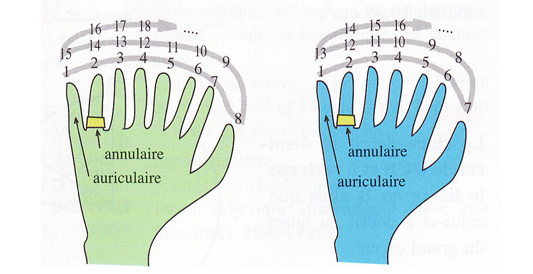
\includegraphics[width=0.9\linewidth]{TP04_plus.png} 
\end{center}
%-------------------------------------------------------------------------------
%-------------------------------------------------------------------------------
\begin{Exercise}
\it Calculer la somme des nombres annulaires compris entre 1 et 2020.
\end{Exercise}
%-------------------------------------------------------------------------------
\begin{Answer}
\begin{lstlisting}
fin = 2020

d7 = 1
sens7 = 1
d8 = 1
sens8 = 1
somme = 0
for i in range(2, fin + 1):
    d7, sens7 = suivant(d7, sens7, 7)
    d8, sens8 = suivant(d8, sens8, 8)
    if d7 == 2 and d8 == 2:
        somme = somme + i
print(somme)
\end{lstlisting}
98882
\newpage
\end{Answer}
%-------------------------------------------------------------------------------
%-------------------------------------------------------------------------------
\subsection{Nombre divisible par morceaux}
%-------------------------------------------------------------------------------
%-------------------------------------------------------------------------------
{\sf Ce problème est le défi Turing 26 : http://apprendre-en-ligne.net/}
%-------------------------------------------------------------------------------
%-------------------------------------------------------------------------------
\begin{Exercise}
\it Trouver un nombre entier $c_1c_2c_3c_4c_5c_6c_7c_8c_9$ composé de tous les chiffres de 1 à 9, tel que $c_1c_2\cdots c_k$ soit divisible par $k$, pour tout $k \in \{1, 2, 3, 4, 5, 6,7, 8,9\}$.

On pourra utiliser \type{permutations} du module \type{itertools}.
\end{Exercise}
%-------------------------------------------------------------------------------
\begin{Answer}
\begin{lstlisting}
from itertools import permutations

def test(suite):
    n = 0
    for k in range(1, 10):
        n = n*10 + suite[k-1]
        if n%k != 0:
            return False, 0
    return True, n

for x in permutations((1, 2, 3, 4, 5, 6, 7, 8, 9)):
    rep, n = test(x)
    if rep:
        print(n)
\end{lstlisting}
381654729
\end{Answer}
%-------------------------------------------------------------------------------
%-------------------------------------------------------------------------------
Plus simplement, pour 3 chiffres, 321 convient.

3 est divisible par 1
32 est divisible par 2
321 est divisible par 3.